\section{Preliminaries}
% ════════════════════════════════════════════════════════════════════════════

\subsection{Multi-objective piecewise-stationary MDP}

\begin{definition}[MO-PS-MDP]
\label{def:mopsmdp}
A \emph{Multi-Objective Piecewise-Stationary MDP} is a sequence of multi-objective MDPs $\{\mathcal{M}_k\}_{k=1}^\infty$ where each $\mathcal{M}_k = (\mathcal{S}, \mathcal{A}, P_k, \mathbf{R}_k, \gamma)$ shares state and action spaces but has distinct:
\begin{itemize}
    \item Transition kernels $P_k : \mathcal{S} \times \mathcal{A} \to \Delta(\mathcal{S})$;
    \item \emph{Vector-valued} reward functions $\mathbf{R}_k : \mathcal{S} \times \mathcal{A} \to \mathbb{R}^m$, where $m$ is the number of objectives;
    \item Discount factor $\gamma \in [0, 1)$ shared across all modes.
\end{itemize}
Regime switches occur at unknown times $t_1 < t_2 < \cdots$.  Between consecutive switches, the MDP is stationary.
\end{definition}

\subsection{Vector-valued Q-functions and metrics}

The Q-function is vector-valued: $\mathbf{Q} : \mathcal{S} \times \mathcal{A} \to \mathbb{R}^m$, where $Q_i(s,a)$ is the expected discounted return for objective $i$.  The function space is equipped with the product $L_\infty$ (sup-norm) metric:
\begin{equation}
    \mathrm{dist}(\mathbf{Q}_1, \mathbf{Q}_2) = \sup_{(s,a) \in \mathcal{S} \times \mathcal{A}} \sup_{i \in \{1,\ldots,m\}} |Q_{1,i}(s,a) - Q_{2,i}(s,a)|.
    \label{eq:dist}
\end{equation}
In Lean~4, this is realized as the nested Pi metric: $\mathcal{S} \times \mathcal{A} \to \mathrm{Fin}\, m \to \mathbb{R}$, where each layer inherits the \texttt{PseudoMetricSpace} instance from Mathlib.

\subsection{Preference-weighted scalarization}

Given a preference weight $w \in \Delta^{m-1}$ (the probability simplex: $w_i \ge 0$, $\sum_i w_i = 1$), the scalarized Q-value is:
\begin{equation}
    Q_w(s,a) = \langle w, \mathbf{Q}(s,a) \rangle = \sum_{i=1}^m w_i \cdot Q_i(s,a).
    \label{eq:scalarize}
\end{equation}
The scalarized greedy value is $V_w(s) = \max_a Q_w(s,a)$. For a fixed vector $\mathbf Q(s,a)$, consider the auxiliary function
\begin{equation}
    f_\eta(w; s,a) = \langle w, \mathbf{Q}(s,a) \rangle - \eta \|w\|^2,
    \label{eq:regularized_scalarize}
\end{equation}
where $\eta>0$ makes this function strictly concave in $w$. This does not imply a bijection between preferences and achievable Pareto returns. If $w$ is a sampled input independent of actor parameters, the quadratic term has zero actor gradient.

\subsection{BAPR: Bayesian Amnesic Piecewise-Robust RL}

BAMOR builds upon the BAPR framework~\cite{Zhang2025BAPR}, which integrates Bayesian Online Change Detection (BOCD)~\cite{Adams2007BOCD} with robust ensemble SAC~\cite{Haarnoja2018SAC, Zhang2025RESAC}.  Key properties we import:
\begin{itemize}
    \item \textbf{BAPR operator:} $\mathcal{T}^{\mathrm{BAPR}}_\rho Q = \sum_h \rho(h) \mathcal{T}_h Q$ is a $\gamma$-contraction when $\rho$ is frozen.
    \item \textbf{Bayesian belief update:} $\rho'(h) = \rho(h) L(h) / Z$ preserves $\rho' \ge 0$ and $\sum_h \rho'(h) = 1$.
    \item \textbf{Counterexample:} Q-dependent beliefs break contraction when $\gamma + \lambda\Delta \ge 1$.
\end{itemize}

\begin{remark}[What changes from BAPR to BAMOR]
\label{rem:bapr_to_bamor}
The extension from BAPR (scalar $Q : \mathcal{S} \times \mathcal{A} \to \mathbb{R}$) to BAMOR (vector $\mathbf{Q} : \mathcal{S} \times \mathcal{A} \to \mathbb{R}^m$) is not a trivial generalization.  It introduces:
\begin{enumerate}
    \item \textbf{Nested metric:} The $L_\infty$ metric on $\mathbb{R}^m$-valued functions requires two layers of Pi-metric unpacking in the contraction proof.
    \item \textbf{Scalarization layer:} An entirely new non-expansiveness proof for the weighted sum, and its composition with component-wise contraction.
    \item \textbf{Weight space geometry:} Lipschitz continuity in $w$, strong concavity, and the anchor-shift theory have no analogue in single-objective BAPR.
    \item \textbf{Component-wise drift:} The Target Cone theory exploits the vector structure of the drift, which collapses to a scalar in BAPR.
\end{enumerate}
\end{remark}


% ════════════════════════════════════════════════════════════════════════════
\section{The BAMOR Framework}
\label{sec:framework}
% ════════════════════════════════════════════════════════════════════════════

\subsection{Mode-conditional multi-objective Bellman operator}

For each environment mode $h \in \mathcal{H}$ (finite, non-empty), we define the mode-conditional multi-objective operator acting on vector-valued Q-functions.

\begin{definition}[Mode-conditional operator --- Lean: \texttt{T\_mode\_mo}]
\label{def:t_mode_mo}
\begin{equation}
    [\mathcal{T}_h \mathbf{Q}](s,a,i) = R_h(s,a,i) + \gamma \left( \sum_{s' \in \mathcal{S}} P_h(s'|s,a) \underbrace{\max_{a' \in \mathcal{A}} Q_i(s',a')}_{V_i^{\mathbf{Q}}(s')} - \lambda_{\mathrm{epi}} \Gamma_{\mathrm{epi},h}(s,a,i) - \kappa_i \right),
    \label{eq:mode_operator}
\end{equation}
where:
\begin{itemize}
    \item $R_h(s,a,i)$ is the reward for objective $i$ under mode $h$;
    \item $V_i^{\mathbf{Q}}(s') = \max_{a'} Q_i(s',a')$ is the per-component value function;
    \item $\Gamma_{\mathrm{epi},h}(s,a,i)$ is the per-objective epistemic penalty from the frozen target ensemble;
    \item $\kappa_i$ is the per-objective aleatoric penalty from frozen critic weights (cf.\ RE-SAC~\cite{Zhang2025RESAC}).
\end{itemize}
\end{definition}

\begin{remark}[Per-objective penalties]
Unlike BAPR (scalar $\kappa$, scalar $\Gamma_{\mathrm{epi}}$), BAMOR uses \emph{per-objective} penalties $\kappa_i$ and $\Gamma_{\mathrm{epi},h}(s,a,i)$.  This allows different objectives to have different aleatoric noise levels and epistemic uncertainty---critical for multi-objective settings where, e.g., speed measurement is noisy but headway measurement is precise.
\end{remark}

\subsection{BAMOR operator: belief-weighted multi-objective mixture}

\begin{definition}[BAMOR operator --- Lean: \texttt{T\_BAMOR}]
\label{def:t_bamor}
The BAMOR operator is the belief-weighted mixture over modes:
\begin{equation}
    [\mathcal{T}^{\mathrm{BAMOR}}_\rho \mathbf{Q}](s,a,i) = \sum_{h \in \mathcal{H}} \rho(h) \cdot [\mathcal{T}_h \mathbf{Q}](s,a,i),
    \label{eq:bamor_operator}
\end{equation}
where $\rho : \mathcal{H} \to [0,1]$ is a belief distribution satisfying $\rho(h) \ge 0$ for all $h$ and $\sum_h \rho(h) = 1$, \textbf{frozen during each Bellman backup}.
\end{definition}

\begin{remark}[Frozen beliefs: necessary, not convenient]
As proven in the BAPR counterexample~\cite{Zhang2025BAPR}, Q-dependent beliefs break contraction.  The frozen-belief design is an essential structural requirement, not a simplification.  The belief is updated \emph{between} backup iterations using the Mahalanobis surprise signal.
\end{remark}

\subsection{Belief-update rules: a separable design choice}
\label{sec:belief_rules}

The contraction proof (\S\ref{sec:contraction}) holds for \emph{any} belief $\rho$ that is frozen across a single backup iteration.  The practical question is how to produce $\rho$ at deployment.  We consider three regimes, in increasing order of algorithmic commitment:

\textbf{(B1) Oracle / mode-labelled belief.}  When the deployment pipeline exposes a mode label $h^\star$ (e.g., a weather code, a traffic-light phase, or a diurnal indicator), set $\rho = \delta_{h^\star}$.  Contraction holds trivially; the cone estimator receives clean per-mode data.

\textbf{(B2) Static uniform belief ($\rho_h = 1/|\mathcal{H}|$).}  When no label is available and we are unwilling to trust an online estimator, freeze the belief at the uniform prior.  The cone estimator then accumulates a \emph{global} anchor that averages over the modes visited during training---a coarse simplification, but one that gives the best empirical results in our high-noise 2-D benchmark (\S\ref{sec:exp_ablation}, variant \texttt{BAMOR-TC}).  Intuitively, the cone-only concentration still filters out low-yield corners of the simplex under the active substrate, which is where most of the wasted exploration under uniform-$w$ sampling occurs.

\textbf{(B3) Online Mahalanobis change-point belief.}  A fully automatic belief update that turns reward residuals into a Mahalanobis $\chi^2$ surprise and triggers a round-robin mode reassignment on threshold crossings:
\begin{align}
    d^2_{\mathrm{Mah}}(\boldsymbol{\xi}, \mathrm{prec}) &= \sum_{i=1}^m \mathrm{prec}_i \cdot \xi_i^2, \qquad
    L(h) = \exp\bigl(-\tfrac{1}{2} d^2_{\mathrm{Mah}}(\boldsymbol{\xi}(h), \mathrm{prec})\bigr).
    \label{eq:mahalanobis}
\end{align}
The Mahalanobis likelihood is strictly positive, so the normalisation $Z = \sum_h \rho(h) L(h) > 0$ automatically (Lean: \texttt{mahalanobis\_normalization\_pos})---this eliminates the ad-hoc $Z > 0$ hypothesis required in generic BAPR.

\textbf{A caveat from our experiments.}  Variant (B3) is elegant in theory and is the mechanism we originally designed.  However, in our current 20-seed 2-objective synthetic benchmark it is not the empirically safest default: enabling the online Mahalanobis detector lowers overall HV from $136.2{\times}10^3$ to $96.9{\times}10^3$ and increases the seed-level std from $23.6{\times}10^3$ to $43.8{\times}10^3$.  The detector also leaves one severe Mode-1 collapse seed ($\mathrm{HV}_{\mathrm{Mode\,1}}<10^3$).  We therefore \emph{do not advocate (B3) as the default recipe}; our reported ``BAMOR'' is variant (B2), and (B3) is evaluated as a secondary ablation to quantify the performance loss caused by a miscalibrated automatic rule.  Designing a well-calibrated online belief update for settings where mode labels are unavailable is an open problem we discuss in \S\ref{sec:limits}.

\subsection{Substrate constraints and Target Cone}
\label{sec:target_cone}

\begin{figure}[t]
\centering
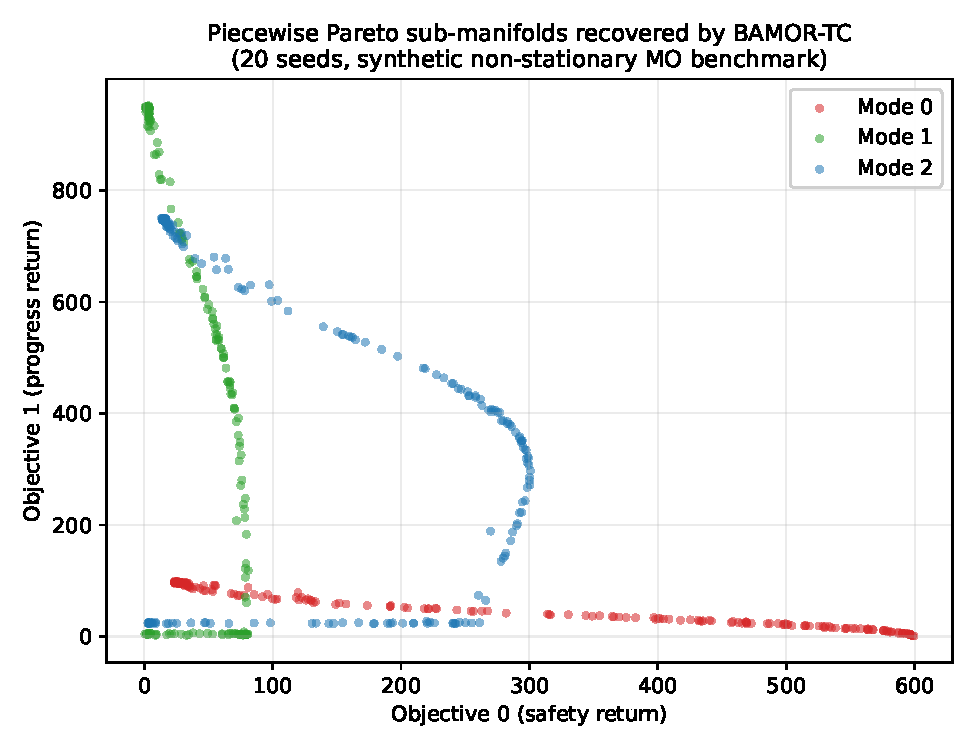
\includegraphics[width=0.78\linewidth]{fig_submfld_hero.pdf}
\caption{The piecewise Pareto sub-manifold structure that BAMOR-TC is designed to exploit, here recovered empirically from $20$ seeds on the synthetic non-stationary MO benchmark.  Each mode's achievable trade-off is a mostly separated, low-dimensional arc: Mode~0 (red) is near-horizontal because progress is strongly capped; Mode~1 (green) is near-vertical because safety is strongly capped; Mode~2 (blue) admits a broader elbow.  The global-smooth-front view is therefore not the right description for this benchmark.  BAMOR's \emph{Target Cone} restricts the weight sampler to the relevant arc per mode (\S\ref{sec:framework}).}
\label{fig:submfld_hero}
\end{figure}

\begin{definition}[Substrate Constraint]
\label{def:substrate}
An environment mode $h$ imposes a \emph{substrate constraint} on objective $i$ if the physical dynamics under mode $h$ bound the achievable improvement in objective $i$ regardless of the policy:
\begin{equation}
    \max_\pi V_i^\pi(s) \le B_{h,i} \quad \text{for all } s \in \mathcal{S},
\end{equation}
where $B_{h,i}$ is a mode-dependent physical ceiling that may be much lower than the ceiling under other modes.  Fig.~\ref{fig:submfld_hero} shows what this looks like in practice: each mode's achievable returns lie on a different arc.
\end{definition}

\begin{definition}[Target Cone --- Lean: \texttt{ModeConeConstraint}]
\label{def:target_cone}
For each mode $h$, the \emph{Target Cone} $\mathcal{C}_h \subset \Delta^{m-1}$ is characterized by:
\begin{itemize}
    \item A \emph{preference anchor} $w_{\mathrm{anchor}}(h) \in \Delta^{m-1}$: the physical center of the cone, satisfying $w_{\mathrm{anchor}}(h,i) \ge 0$ and $\sum_i w_{\mathrm{anchor}}(h,i) = 1$;
    \item A \emph{cone radius} $r_h > 0$: $\mathcal{C}_h = \{w \in \Delta^{m-1} : \|w - w_{\mathrm{anchor}}(h)\|_2 \le r_h\}$.
\end{itemize}
Weights outside $\mathcal{C}_h$ remain valid preferences. The cone is a chosen training-allocation region, not a characterization of all achievable returns.
\end{definition}

\begin{example}[Target Cones for bus transit]
\label{ex:cones}
For an illustrative two-objective setting with $m=2$:
\begin{center}
\begin{tabular}{lccc}
\toprule
\textbf{Mode} & $w_{\mathrm{anchor}}$ & \textbf{Cone interval} & \textbf{Physical reason} \\
\midrule
Normal & $(0.5, 0.5)$ & $w_{\mathrm{headway}} \in [0.3, 0.7]$ & Free trade-off \\
Severe congestion & $(0.95, 0.05)$ & $w_{\mathrm{headway}} \in [0.85, 1.0]$ & Speed ceiling hit \\
Demand surge & $(0.2, 0.8)$ & $w_{\mathrm{headway}} \in [0.1, 0.4]$ & Must move passengers \\
\bottomrule
\end{tabular}
\end{center}
\end{example}

\begin{definition}[Belief-weighted anchor --- Lean: \texttt{belief\_weighted\_anchor}]
\label{def:belief_anchor}
The belief-weighted anchor aggregates mode-specific anchors:
\begin{equation}
    \tilde{w}_i = \sum_{h \in \mathcal{H}} \rho(h) \cdot w_{\mathrm{anchor}}(h, i).
    \label{eq:belief_anchor}
\end{equation}
When $\rho$ concentrates on mode $h_0$ (after surprise detection), $\tilde{w} \approx w_{\mathrm{anchor}}(h_0)$.  During uncertainty (diffuse $\rho$), it smoothly interpolates.
\end{definition}

\subsection{Anchor-shifted regularization}
\label{sec:anchor_reg}

For the auxiliary scalarization analysis, shift the quadratic center to a fixed anchor:
\begin{equation}
    f_{\mathrm{anchor}}(w; s,a) = \langle w, \mathbf{Q}(s,a) \rangle - \eta \|w - \tilde{w}\|^2.
    \label{eq:anchor_reg}
\end{equation}
The curvature with respect to $w$ is unchanged (Theorem~\ref{thm:anchor_concavity}). In the implemented actor update, $w$ and the anchor are fixed inputs, so this term has no actor gradient and is omitted.

\subsection{Context-aware weight sampling}
\label{sec:sampling}

The current BAMOR-TC sampler concentrates a Dirichlet distribution around the estimated anchor:
\begin{equation}
    w\sim\mathrm{Dirichlet}(\alpha),\qquad
    \alpha_i=\kappa_{\mathrm{eff}}\tilde w_i+10^{-3},
\end{equation}
where the effective concentration is scaled by the estimated cone radius. This distribution has full simplex-interior support; it is not uniform sampling from, or hard truncation to, $\mathcal C_h$. A radius therefore specifies concentration, not a guaranteed support boundary. BAMOR-v23 instead uses the selected arm's uniform, stratified, mixed or extreme-preference sampler.

\section{Theoretical Analysis}
\label{sec:theory}
% ════════════════════════════════════════════════════════════════════════════

All theorems in this section are machine-verified in Lean~4/Mathlib with no \texttt{sorry}.  Full proof details with complete derivations are in Appendix~\ref{app:contraction}--\ref{app:improvement}.  We state each result with proof sketches that highlight the key mathematical moves.

\subsection{BAMOR is a gamma-contraction (Parts I--VI)}
\label{sec:contraction}

The proof proceeds bottom-up: per-component max properties $\to$ per-mode properties $\to$ mixture properties $\to$ Banach fixed point.

\subsubsection{Component-wise max properties}

\begin{lemma}[Component-wise max is 1-Lipschitz --- Lean: \texttt{max\_over\_a\_comp\_nonexpansive}]
\label{lem:max_lip}
If $|Q_{1,i}(s,a) - Q_{2,i}(s,a)| \le \varepsilon$ for all $s,a,i$, then $|V_i^{\mathbf{Q}_1}(s) - V_i^{\mathbf{Q}_2}(s)| \le \varepsilon$ for all $s,i$.
\end{lemma}

\begin{proof}
For the upper bound: for any action $a$, $Q_{1,i}(s,a) \le Q_{2,i}(s,a) + \varepsilon \le V_i^{\mathbf{Q}_2}(s) + \varepsilon$.  Taking $\max_a$ gives $V_i^{\mathbf{Q}_1}(s) \le V_i^{\mathbf{Q}_2}(s) + \varepsilon$.  Symmetrically for the lower bound.  The Lean proof proceeds via \texttt{Finset.sup'\_le} applied to the finite action space.
\end{proof}

\subsubsection{Per-mode contraction}

\begin{lemma}[Per-mode pointwise bound --- Lean: \texttt{t\_mode\_mo\_pointwise\_bound}]
\label{lem:mode_bound}
If $\mathrm{dist}(\mathbf{Q}_1, \mathbf{Q}_2) \le \varepsilon$, then $|[\mathcal{T}_h \mathbf{Q}_1](s,a,i) - [\mathcal{T}_h \mathbf{Q}_2](s,a,i)| \le \gamma\varepsilon$ for all $h,s,a,i$.
\end{lemma}

\begin{proof}
The frozen penalties ($R_h$, $\Gamma_{\mathrm{epi},h}$, $\kappa_i$) cancel in the difference.  By Lemma~\ref{lem:max_lip}: $|V_i^{\mathbf{Q}_1}(s') - V_i^{\mathbf{Q}_2}(s')| \le \varepsilon$.  Then:
\begin{align}
    |[\mathcal{T}_h \mathbf{Q}_1 - \mathcal{T}_h \mathbf{Q}_2](s,a,i)| &= \gamma \left|\sum_{s'} P_h(s'|s,a)(V_i^{\mathbf{Q}_1}(s') - V_i^{\mathbf{Q}_2}(s'))\right| \notag \\
    &\le \gamma \sum_{s'} P_h(s'|s,a) |V_i^{\mathbf{Q}_1}(s') - V_i^{\mathbf{Q}_2}(s')| \quad \text{(triangle, $P_h \ge 0$)} \notag \\
    &\le \gamma \sum_{s'} P_h(s'|s,a) \cdot \varepsilon = \gamma\varepsilon \cdot \underbrace{\sum_{s'} P_h(s'|s,a)}_{=1}. \qedhere
\end{align}
\end{proof}

\subsubsection{Main contraction theorem}

\begin{theorem}[BAMOR gamma-contraction --- Lean: \texttt{bamor\_contraction}]
\label{thm:bamor_contraction}
Under (A0)--(A4), the BAMOR operator satisfies:
\begin{equation}
    \mathrm{dist}(\mathcal{T}^{\mathrm{BAMOR}}_\rho \mathbf{Q}_1, \mathcal{T}^{\mathrm{BAMOR}}_\rho \mathbf{Q}_2) \le \gamma \cdot \mathrm{dist}(\mathbf{Q}_1, \mathbf{Q}_2).
\end{equation}
\end{theorem}

\begin{proof}
Let $\varepsilon = \mathrm{dist}(\mathbf{Q}_1, \mathbf{Q}_2)$.  We need to show $\mathrm{dist}(\mathcal{T}\mathbf{Q}_1, \mathcal{T}\mathbf{Q}_2) \le \gamma\varepsilon$.  By Eq.~\eqref{eq:dist}, this requires showing $|[\mathcal{T}\mathbf{Q}_1](s,a,i) - [\mathcal{T}\mathbf{Q}_2](s,a,i)| \le \gamma\varepsilon$ for all $(s,a,i)$.

Expanding the BAMOR operator:
\begin{align}
    &|[\mathcal{T}^{\mathrm{BAMOR}}_\rho \mathbf{Q}_1](s,a,i) - [\mathcal{T}^{\mathrm{BAMOR}}_\rho \mathbf{Q}_2](s,a,i)| \notag \\
    &= \left|\sum_{h} \rho(h) \left([\mathcal{T}_h \mathbf{Q}_1](s,a,i) - [\mathcal{T}_h \mathbf{Q}_2](s,a,i)\right)\right| \notag \\
    &\le \sum_{h} \rho(h) \left|[\mathcal{T}_h \mathbf{Q}_1](s,a,i) - [\mathcal{T}_h \mathbf{Q}_2](s,a,i)\right| \quad \text{(triangle inequality, $\rho(h) \ge 0$ by (A3))} \notag \\
    &\le \sum_{h} \rho(h) \cdot \gamma\varepsilon \quad \text{(per-mode bound, Lemma~\ref{lem:mode_bound})} \notag \\
    &= \gamma\varepsilon \cdot \sum_{h} \rho(h) = \gamma\varepsilon. \quad \text{($\sum \rho = 1$ by (A4))}
\end{align}

The Lean proof (function \texttt{bamor\_dist\_le}) proceeds by:
\begin{enumerate}
    \item Setting $\varepsilon := \mathrm{dist}(\mathbf{Q}_1, \mathbf{Q}_2)$ and showing $0 \le \varepsilon$;
    \item Applying \texttt{dist\_pi\_le\_iff} twice to unpack the nested Pi metric, reducing to pointwise bounds;
    \item Extracting pointwise bounds $|Q_{1,i}(s,a) - Q_{2,i}(s,a)| \le \varepsilon$ from the dist assumption;
    \item Applying the mode-bound lemma and the triangle-inequality/normalization argument;
    \item Taking the supremum over $(s,a,i)$ via \texttt{dist\_pi\_le\_iff} in the reverse direction.
\end{enumerate}
The existential form $\exists k < 1, \forall \mathbf{Q}_1\,\mathbf{Q}_2,\, \mathrm{dist}(\mathcal{T}\mathbf{Q}_1, \mathcal{T}\mathbf{Q}_2) \le k \cdot \mathrm{dist}(\mathbf{Q}_1, \mathbf{Q}_2)$ follows by witnessing $k := \gamma$ and $\gamma < 1$.
\end{proof}

\subsubsection{Blackwell conditions (Lean: Parts I)}

For completeness and to bridge to the classical theory, we also verify both Blackwell conditions:

\begin{lemma}[BAMOR monotonicity --- Blackwell (i) --- Lean: \texttt{bamor\_monotonicity}]
If $\mathbf{Q}_1 \le \mathbf{Q}_2$ pointwise, then $\mathcal{T}^{\mathrm{BAMOR}}_\rho \mathbf{Q}_1 \le \mathcal{T}^{\mathrm{BAMOR}}_\rho \mathbf{Q}_2$ pointwise.
\end{lemma}

\begin{lemma}[BAMOR discounting --- Blackwell (ii) --- Lean: \texttt{bamor\_discounting}]
For any constant vector $\mathbf{c} \in \mathbb{R}^m$: $\mathcal{T}^{\mathrm{BAMOR}}_\rho(\mathbf{Q} + \mathbf{c}) = \mathcal{T}^{\mathrm{BAMOR}}_\rho \mathbf{Q} + \gamma \mathbf{c}$.
\end{lemma}

\begin{proof}
The discounting proof is where $\sum_h \rho(h) = 1$ (A4) is essential.  Per-mode: $\mathcal{T}_h(\mathbf{Q} + \mathbf{c})(s,a,i) = \mathcal{T}_h\mathbf{Q}(s,a,i) + \gamma c_i$ (because $\max_a (Q_i(s,a) + c_i) = \max_a Q_i(s,a) + c_i$ and $\sum_{s'} P_h = 1$).  Mixing: $\sum_h \rho(h)(\mathcal{T}_h\mathbf{Q}(s,a,i) + \gamma c_i) = \mathcal{T}^{\mathrm{BAMOR}}\mathbf{Q}(s,a,i) + \gamma c_i \cdot \sum_h \rho(h) = \mathcal{T}^{\mathrm{BAMOR}}\mathbf{Q}(s,a,i) + \gamma c_i$.
\end{proof}

\subsubsection{Banach fixed point (Part VI)}

\begin{corollary}[Existence and uniqueness]
\label{cor:fixed_point}
$\mathcal{T}^{\mathrm{BAMOR}}_\rho$ has a unique fixed point $\mathbf Q^*$ in the finite-dimensional vector-value space. The independent coordinate maximizations do not imply joint achievability by one policy.

For example, with one state, zero penalties, and actions with rewards $(1,0)$ and $(0,1)$, the componentwise optimal state value is $(1/(1-\gamma),1/(1-\gamma))$. Every realizable policy has the sum of its two state-value coordinates equal to $1/(1-\gamma)$. Thus the componentwise fixed-point construction must not be identified with an achievable Pareto-optimal policy.
\end{corollary}

\begin{proof}
\textbf{Uniqueness:} If $\mathcal{T}\mathbf{Q}_1 = \mathbf{Q}_1$ and $\mathcal{T}\mathbf{Q}_2 = \mathbf{Q}_2$, then $\mathrm{dist}(\mathbf{Q}_1, \mathbf{Q}_2) = \mathrm{dist}(\mathcal{T}\mathbf{Q}_1, \mathcal{T}\mathbf{Q}_2) \le \gamma \mathrm{dist}(\mathbf{Q}_1, \mathbf{Q}_2)$.  Since $\gamma < 1$ and $\mathrm{dist} \ge 0$: $(1 - \gamma)\mathrm{dist} \le 0$, forcing $\mathrm{dist} = 0$.

\textbf{Existence:} The Lean proof bridges to Mathlib's \texttt{ContractingWith.exists\_fixedPoint}, starting from $\mathbf{Q}_0 = 0$.  The key steps: (i)~\texttt{bamor\_lipschitzWith} shows Lipschitz constant $\gamma$; (ii)~\texttt{bamor\_contractingWith} packages this with $\gamma < 1$; (iii)~the finite type ensures \texttt{edist} from $\mathbf{Q}_0$ to $\mathcal{T}\mathbf{Q}_0$ is finite.
\end{proof}

\subsubsection{Contraction after belief update (Parts II, IV)}

\begin{corollary}[Post-update contraction --- Lean: \texttt{bamor\_contraction\_after\_update}]
If $\rho$ is updated to $\rho'$ via Bayesian update with $Z > 0$, then $\mathcal{T}^{\mathrm{BAMOR}}_{\rho'}$ is a $\gamma$-contraction.
\end{corollary}

\begin{corollary}[Mahalanobis contraction --- Lean: \texttt{bamor\_contraction\_mahalanobis}]
\label{cor:mahalanobis}
With Mahalanobis likelihood, the $Z > 0$ requirement is automatically satisfied from prior support ($\exists h, \rho(h) > 0$), providing a stronger guarantee than generic BAPR.
\end{corollary}


\subsection{Scalarized contraction and weight sensitivity (Parts VII--VIII)}
\label{sec:scalarized}

\begin{theorem}[Scalarized BAMOR contraction --- Lean: \texttt{scalarized\_bamor\_contraction}]
\label{thm:scalarized_contraction}
For any $w \in \Delta^{m-1}$ and any $(s,a)$:
\begin{equation}
    |\langle w, \mathcal{T}^{\mathrm{BAMOR}}_\rho \mathbf{Q}_1(s,a) \rangle - \langle w, \mathcal{T}^{\mathrm{BAMOR}}_\rho \mathbf{Q}_2(s,a) \rangle| \le \gamma \cdot \mathrm{dist}(\mathbf{Q}_1, \mathbf{Q}_2).
\end{equation}
\end{theorem}

\begin{proof}
This composes two results:
\begin{enumerate}
    \item \textbf{Part I (contraction):} $|[\mathcal{T}\mathbf{Q}_1](s,a,i) - [\mathcal{T}\mathbf{Q}_2](s,a,i)| \le \gamma\varepsilon$ for all $i$;
    \item \textbf{Part III (non-expansiveness):} $|\sum_i w_i (f_i - g_i)| \le \sum_i w_i |f_i - g_i| \le \max_i |f_i - g_i|$ when $w \ge 0, \sum w_i = 1$.
\end{enumerate}
Combining: $|\langle w, \mathcal{T}\mathbf{Q}_1(s,a) - \mathcal{T}\mathbf{Q}_2(s,a) \rangle| \le \gamma\varepsilon$.
\end{proof}

\begin{remark}[Why this matters]
Theorem~\ref{thm:scalarized_contraction} bounds the scalarized output difference by $\gamma$ times the vector sup-norm input difference. It is not a contraction statement in the scalarized-input pseudometric, nor a convergence result for preference-conditioned neural control.
\end{remark}

\begin{lemma}[Weight Lipschitz --- Lean: \texttt{scalarize\_lipschitz\_in\_w}]
\label{lem:weight_lipschitz}
For Q-values bounded by $B$ ($|Q_i(s,a)| \le B$ for all $s,a,i$):
\begin{equation}
    |\langle w_1, \mathbf{Q}(s,a) \rangle - \langle w_2, \mathbf{Q}(s,a) \rangle| \le B \cdot \|w_1 - w_2\|_1.
\end{equation}
\end{lemma}

\begin{proof}
$|\sum_i (w_{1,i} - w_{2,i}) Q_i(s,a)| \le \sum_i |w_{1,i} - w_{2,i}| \cdot |Q_i(s,a)| \le B \sum_i |w_{1,i} - w_{2,i}|$.
\end{proof}

\begin{corollary}[Pareto value Lipschitz --- Lean: \texttt{pareto\_val\_lipschitz\_in\_w}]
$|V_{w_1}(s) - V_{w_2}(s)| \le B \cdot \|w_1 - w_2\|_1$.
\end{corollary}

This result quantifies the ``nearby preferences $\Rightarrow$ nearby values'' property, justifying the cone-restricted sampling: if the sampled $w$ is within radius $r_h$ of the anchor, the resulting value differs by at most $B \cdot 2r_h$ from the anchor's value.


\subsection{Strong concavity and anchor-shifted regularization (Parts IX, XI, XIII)}
\label{sec:anchor}

\subsubsection{Auxiliary quadratic scalarization (Part IX)}

\begin{theorem}[Strong concavity --- Lean: \texttt{regularized\_scalarize\_strongly\_concave}]
\label{thm:strong_concavity}
For any $\eta, t \in \mathbb{R}$ and any $w_1, w_2$:
\begin{equation}
    f_\eta(tw_1 + (1{-}t)w_2) \ge t \cdot f_\eta(w_1) + (1{-}t) \cdot f_\eta(w_2) + \eta t(1{-}t)\|w_1 - w_2\|^2,
\end{equation}
where $f_\eta(w) = \langle w, \mathbf{Q}(s,a) \rangle - \eta\|w\|^2$.
\end{theorem}

\begin{proof}
The proof uses two ingredients:
\begin{enumerate}
    \item \textbf{Linearity of scalarization:} $\langle tw_1 + (1{-}t)w_2, \mathbf{Q} \rangle = t\langle w_1, \mathbf{Q} \rangle + (1{-}t)\langle w_2, \mathbf{Q} \rangle$ (Lean: \texttt{scalarize\_affine\_in\_w}).
    \item \textbf{Parallelogram identity:} $\|tw_1 + (1{-}t)w_2\|^2 + t(1{-}t)\|w_1 - w_2\|^2 = t\|w_1\|^2 + (1{-}t)\|w_2\|^2$ (Lean: \texttt{weight\_norm\_sq\_convex\_identity}).
\end{enumerate}
Substituting (1) and rearranging (2) into the definition of $f_\eta$:
\begin{align}
    f_\eta(tw_1 + (1{-}t)w_2) &= t\langle w_1, \mathbf{Q} \rangle + (1{-}t)\langle w_2, \mathbf{Q} \rangle - \eta\|tw_1 + (1{-}t)w_2\|^2 \\
    &= t\langle w_1, \mathbf{Q} \rangle + (1{-}t)\langle w_2, \mathbf{Q} \rangle - \eta(t\|w_1\|^2 + (1{-}t)\|w_2\|^2 - t(1{-}t)\|w_1 - w_2\|^2) \\
    &= tf_\eta(w_1) + (1{-}t)f_\eta(w_2) + \eta t(1{-}t)\|w_1 - w_2\|^2.
\end{align}
The gap $\eta t(1{-}t)\|w_1 - w_2\|^2 > 0$ when $\eta > 0$, $t \in (0,1)$, $w_1 \ne w_2$, guaranteeing strict concavity.
\end{proof}

\subsubsection{Anchor-shifted regularization (Part XI)}

\begin{theorem}[Anchor-shifted strong concavity]
\label{thm:anchor_concavity}
\emph{Lean: \texttt{anchor\_regularized\_strongly\_concave}.}

Shifting the regularization center to any $w_{\mathrm{anchor}}$ preserves the \textbf{identical} strong concavity gap:
\begin{equation}
    f_{\mathrm{anchor}}(tw_1 + (1{-}t)w_2) \ge tf_{\mathrm{anchor}}(w_1) + (1{-}t)f_{\mathrm{anchor}}(w_2) + \eta t(1{-}t)\|w_1 - w_2\|^2,
\end{equation}
where $f_{\mathrm{anchor}}(w) = \langle w, \mathbf{Q}(s,a) \rangle - \eta\|w - w_{\mathrm{anchor}}\|^2$.
\end{theorem}

\begin{proof}
The key insight is a change of variables: let $u = w - w_{\mathrm{anchor}}$.
\begin{enumerate}
    \item The convex combination shifts: $t w_1 + (1{-}t)w_2 - w_{\mathrm{anchor}} = t(w_1 - w_{\mathrm{anchor}}) + (1{-}t)(w_2 - w_{\mathrm{anchor}}) = tu_1 + (1{-}t)u_2$.
    \item Apply the parallelogram identity to $u_1, u_2$: $$\|tu_1 + (1{-}t)u_2\|^2 = t\|u_1\|^2 + (1{-}t)\|u_2\|^2 - t(1{-}t)\|u_1 - u_2\|^2.$$
    \item The anchor cancels in the difference: $u_1 - u_2 = (w_1 - w_{\mathrm{anchor}}) - (w_2 - w_{\mathrm{anchor}}) = w_1 - w_2$.
\end{enumerate}
Therefore $\|u_1 - u_2\|^2 = \|w_1 - w_2\|^2$, and the gap is \emph{identical} to the origin-centered case.  Geometrically: the Hessian $\nabla^2_w f_{\mathrm{anchor}} = -2\eta I$ is constant (translation-invariant).
\end{proof}

\begin{remark}[Physical significance]
This theorem concerns the curvature of an auxiliary function of $w$. It neither supplies an actor gradient for a sampled fixed weight nor establishes coverage of the Pareto front.
\end{remark}

\subsubsection{Mode Cone formalization and belief-anchor validity (Part XIII)}

\begin{theorem}[Belief-anchor is a valid preference --- Lean: \texttt{belief\_anchor\_valid\_preference}]
\label{thm:belief_anchor}
If each mode's anchor lies on $\Delta^{m-1}$ and $\rho$ is a valid belief, then the belief-weighted anchor $\tilde{w}$ (Eq.~\ref{eq:belief_anchor}) satisfies $\tilde{w}_i \ge 0$ for all $i$ and $\sum_i \tilde{w}_i = 1$.
\end{theorem}

\begin{proof}
Non-negativity: $\tilde{w}_i = \sum_h \rho(h) w_{\mathrm{anchor}}(h,i) \ge 0$ since each term is a product of non-negatives.  Normalization:
\begin{align}
    \sum_i \tilde{w}_i &= \sum_i \sum_h \rho(h) w_{\mathrm{anchor}}(h,i) = \sum_h \rho(h) \underbrace{\sum_i w_{\mathrm{anchor}}(h,i)}_{=1} = \sum_h \rho(h) = 1. \qedhere
\end{align}
\end{proof}

\begin{theorem}[Pipeline preserves strong concavity]
The anchor-shifted strong concavity (Theorem~\ref{thm:anchor_concavity}) holds when $w_{\mathrm{anchor}} = \tilde{w}$, proving that the entire BAMOR pipeline---surprise detection $\to$ belief update $\to$ anchor computation $\to$ regularized scalarization---preserves strong concavity at every step, for any valid belief $\rho$.
\end{theorem}


\subsection{Localized scalarized tracking bounds (Parts X, XII--XV)}
\label{sec:tracking}

This section formalizes when localized preference or operator choices improve a non-stationary tracking bound.  The comparison is conditional: the localized scalarized drift must be no larger than the global worst-component drift.  The result explains Target-Cone sampling and also applies to other selected operators that induce aligned non-negative preference weights.

\subsubsection{Global tracking under non-stationarity (Part X)}

\begin{theorem}[BAMOR robust tracking --- Lean: \texttt{bamor\_robust\_tracking}]
\label{thm:robust_tracking}
Given a sequence of $\gamma$-contractions $\{T_n\}$ (each from BAMOR with a different belief $\rho_n$) and bounded per-step target drift $\Delta$:
\begin{equation}
    \mathrm{dist}(\mathbf{Q}_n, \mathbf{Q}^*_n) \le \gamma^n \cdot D_0 + \frac{\Delta}{1 - \gamma},
    \label{eq:global_tracking}
\end{equation}
where $D_0 = \mathrm{dist}(\mathbf{Q}_0, \mathbf{Q}^*_0)$.
\end{theorem}

\begin{proof}
\textbf{Step 1 (Per-step recursion, Lean: \texttt{time\_varying\_contraction\_step}):}
\begin{align}
    \mathrm{dist}(\mathbf{Q}_{n+1}, \mathbf{Q}^*_{n+1}) &= \mathrm{dist}(T_n(\mathbf{Q}_n), \mathbf{Q}^*_{n+1}) \\
    &\le \mathrm{dist}(T_n(\mathbf{Q}_n), T_n(\mathbf{Q}^*_n)) + \mathrm{dist}(T_n(\mathbf{Q}^*_n), \mathbf{Q}^*_{n+1}) \quad \text{(triangle)} \\
    &\le \gamma \cdot \mathrm{dist}(\mathbf{Q}_n, \mathbf{Q}^*_n) + \Delta. \quad \text{(contraction + drift)}
\end{align}

\textbf{Step 2 (Induction, Lean: \texttt{anytime\_tracking\_bound}):} With the recursion $e(n+1) \le \gamma e(n) + \Delta$, induction gives $e(n) \le \gamma^n e(0) + \Delta/(1{-}\gamma)$, using $\gamma \cdot \Delta/(1{-}\gamma) + \Delta = \Delta/(1{-}\gamma)$.
\end{proof}

\subsubsection{Scalarized drift suppression (Part XII)}

\begin{definition}[Component-wise drift --- Lean: \texttt{pointwise\_drift\_bound}]
$\Delta_{\mathrm{vec}} \in \mathbb{R}^m_{\ge 0}$ satisfies $|Q_{1,i}(s,a) - Q_{2,i}(s,a)| \le \Delta_{\mathrm{vec},i}$ for all $s,a,i$.
\end{definition}

\begin{lemma}[Scalarized drift suppression --- Lean: \texttt{scalarized\_drift\_suppression}]
\label{lem:drift_suppression}
For $w \ge 0$:
\begin{equation}
    |\langle w, \mathbf{Q}_1(s,a) - \mathbf{Q}_2(s,a) \rangle| \le \sum_{i=1}^m w_i \cdot \Delta_{\mathrm{vec},i} = \langle w, \Delta_{\mathrm{vec}} \rangle.
\end{equation}
\end{lemma}

\begin{proof}
\begin{align}
    \left|\sum_i w_i(Q_{1,i} - Q_{2,i})\right| &\le \sum_i |w_i(Q_{1,i} - Q_{2,i})| = \sum_i w_i |Q_{1,i} - Q_{2,i}| \quad (\text{since } w_i \ge 0) \\
    &\le \sum_i w_i \Delta_{\mathrm{vec},i}. \qedhere
\end{align}
\end{proof}

\begin{example}[Drift suppression in practice]
\label{ex:drift}
Consider a mode switch from normal ($Q^*_{\mathrm{headway}} = 50$, $Q^*_{\mathrm{speed}} = 100$) to congested ($Q^*_{\mathrm{headway}} = 45$, $Q^*_{\mathrm{speed}} = 10$).  Then $\Delta_{\mathrm{vec}} = (5, 90)$ and $\Delta_{\mathrm{global}} = \max(5, 90) = 90$.

With a Target-Cone-aligned weight $w = (0.95, 0.05)$:
\begin{equation}
    \Delta_{\mathrm{local}} = 0.95 \times 5 + 0.05 \times 90 = 4.75 + 4.5 = 9.25.
\end{equation}
The suppression ratio: $\Delta_{\mathrm{local}} / \Delta_{\mathrm{global}} = 9.25 / 90 \approx 10.3\%$.  The scalarized drift is compressed to about one-tenth of the global drift.

With $\gamma = 0.99$:
\begin{equation}
    \text{Naive bound: } \frac{90}{0.01} = 9000, \quad \text{BAMOR bound: } 9.25 + 0.99 \times 9000 = 9.25 + 8910 = 8919.25.
\end{equation}
The improvement is $9000 - 8919.25 = 80.75$, corresponding to $\Delta_{\mathrm{global}} - \Delta_{\mathrm{local}} = 90 - 9.25 = 80.75$.  $\checkmark$
\end{example}

\subsubsection{Single-step Target Cone bound (Part XII)}

\begin{theorem}[Target-Cone single-step --- Lean: \texttt{time\_varying\_scalarized\_contraction\_step}]
\label{thm:single_step_tc}
\begin{equation}
    |\langle w, \mathbf{Q}_{n+1}(s,a) \rangle - \langle w, \mathbf{Q}^*_{n+1}(s,a) \rangle| \le \gamma \cdot \mathrm{dist}(\mathbf{Q}_n, \mathbf{Q}^*_n) + \langle w, \Delta_{\mathrm{vec}} \rangle.
\end{equation}
\end{theorem}

\begin{proof}
Decompose via triangle inequality:
\begin{align}
    &|\langle w, T_n(\mathbf{Q}_n)(s,a) \rangle - \langle w, \mathbf{Q}^*_{n+1}(s,a) \rangle| \notag \\
    &\le \underbrace{|\langle w, T_n(\mathbf{Q}_n)(s,a) \rangle - \langle w, T_n(\mathbf{Q}^*_n)(s,a) \rangle|}_{\text{Term 1: contraction}} + \underbrace{|\langle w, T_n(\mathbf{Q}^*_n)(s,a) \rangle - \langle w, \mathbf{Q}^*_{n+1}(s,a) \rangle|}_{\text{Term 2: drift}}.
\end{align}

\textbf{Term 1:} By scalarize non-expansiveness (Lemma~\ref{lem:scalarize_nonexp} from Part III) applied to $T_n(\mathbf{Q}_n)$ and $T_n(\mathbf{Q}^*_n)$: $\le \mathrm{dist}(T_n(\mathbf{Q}_n), T_n(\mathbf{Q}^*_n)) \le \gamma \mathrm{dist}(\mathbf{Q}_n, \mathbf{Q}^*_n)$.

\textbf{Term 2:} By scalarized drift suppression (Lemma~\ref{lem:drift_suppression}): $\le \langle w, \Delta_{\mathrm{vec}} \rangle$.
\end{proof}

\subsubsection{End-to-end Target Cone bound (Part XIV)}

\begin{theorem}[Target Cone multi-step tracking --- Lean: \texttt{target\_cone\_multistep\_tracking}]
\label{thm:target_cone}
For $n \ge 1$, with Target-Cone-aligned weight $w$:
\begin{equation}
    |\langle w, \mathbf{Q}_n(s,a) \rangle - \langle w, \mathbf{Q}^*_n(s,a) \rangle| \le \gamma^n D_0 + \gamma \cdot \frac{\Delta_g}{1{-}\gamma} + \langle w, \Delta_{\mathrm{vec}} \rangle.
    \label{eq:capstone}
\end{equation}
\end{theorem}

\begin{proof}
Write $n = k + 1$ (since $n \ge 1$).

\textbf{Step 1 (Part XII):} Apply Theorem~\ref{thm:single_step_tc} at step $k$:
\begin{equation}
    |\langle w, \mathbf{Q}_{k+1} \rangle - \langle w, \mathbf{Q}^*_{k+1} \rangle| \le \gamma \cdot \mathrm{dist}(\mathbf{Q}_k, \mathbf{Q}^*_k) + \Delta_{\mathrm{local}}.
\end{equation}

\textbf{Step 2 (Part X):} Substitute the global tracking bound at step $k$:
\begin{equation}
    \mathrm{dist}(\mathbf{Q}_k, \mathbf{Q}^*_k) \le \gamma^k D_0 + \frac{\Delta_g}{1{-}\gamma}.
\end{equation}

\textbf{Step 3 (Compose):}
\begin{align}
    \gamma \left(\gamma^k D_0 + \frac{\Delta_g}{1{-}\gamma}\right) + \Delta_{\mathrm{local}} = \gamma^{k+1} D_0 + \gamma \cdot \frac{\Delta_g}{1{-}\gamma} + \Delta_{\mathrm{local}}. \qedhere
\end{align}
\end{proof}

\begin{remark}[Steady-state analysis]
As $n \to \infty$, the transient $\gamma^n D_0 \to 0$.  The residual tracking error is:
\begin{equation}
    \text{BAMOR: } \Delta_{\mathrm{local}} + \gamma \cdot \frac{\Delta_g}{1{-}\gamma}, \qquad \text{Naive: } \frac{\Delta_g}{1{-}\gamma}.
\end{equation}
\end{remark}

\subsubsection{Improvement quantification (Part XV)}

\begin{theorem}[Target Cone improvement --- Lean: \texttt{target\_cone\_improvement}]
\label{thm:improvement}
\begin{equation}
    \underbrace{\frac{\Delta_g}{1{-}\gamma}}_{\text{Naive}} - \underbrace{\left(\Delta_{\mathrm{local}} + \gamma \cdot \frac{\Delta_g}{1{-}\gamma}\right)}_{\text{BAMOR}} = \Delta_g - \Delta_{\mathrm{local}}.
\end{equation}
\end{theorem}

\begin{proof}
$\frac{\Delta_g}{1{-}\gamma} - \Delta_{\mathrm{local}} - \gamma \cdot \frac{\Delta_g}{1{-}\gamma} = (1{-}\gamma) \cdot \frac{\Delta_g}{1{-}\gamma} - \Delta_{\mathrm{local}} = \Delta_g - \Delta_{\mathrm{local}}$.
\end{proof}

\begin{corollary}[Non-negative improvement --- Lean: \texttt{target\_cone\_improvement\_nonneg}]
$\Delta_{\mathrm{local}} + \gamma \Delta_g/(1{-}\gamma) \le \Delta_g/(1{-}\gamma)$ whenever $\Delta_{\mathrm{local}} \le \Delta_g$.
\end{corollary}

\begin{corollary}[Full suppression --- Lean: \texttt{full\_suppression\_ratio}]
When $\Delta_{\mathrm{local}} = 0$, the localized residual bound is $\gamma\Delta_g/(1{-}\gamma)$. For $\gamma=0.99$, this is $99\%$ of the global residual bound, a $1\%$ reduction. This concerns upper bounds, not the ratio of actual errors.
\end{corollary}

\begin{center}
\begin{tabular}{lccc}
\toprule
\textbf{Scenario} & $\Delta_{\mathrm{local}}/\Delta_g$ & \textbf{BAMOR bound} & \textbf{Improvement} \\
\midrule
Equal local/global drift & $1.0$ & $\Delta_g/(1{-}\gamma)$ & $0$ \\
Partial (Example~\ref{ex:drift}) & $0.103$ & $0.103\Delta_g + 0.99\Delta_g/(1{-}\gamma)$ & $0.897\Delta_g$ \\
Full ($\Delta_{\mathrm{local}} = 0$) & $0.0$ & $\gamma\Delta_g/(1{-}\gamma)$ & $\Delta_g$ \\
\bottomrule
\end{tabular}
\end{center}

\begin{remark}[Relation to global-simplex baselines]
\begin{itemize}
    \item \textbf{CAPQL:} Its standard guarantee is stationary; it does not provide a mode-switch tracking bound.
    \item \textbf{GPI-PD and MOSAC:} Standard implementations sample broadly over $\Delta^{m-1}$ and therefore do not target the local-drift term explicitly.
    \item \textbf{\texttt{morl-baselines}:} CAPQL's \texttt{WeightSamplerAngle} uses a fixed $22.5^\circ$ cone centered on the uniform direction; this is a useful numerical device but not an environment-adaptive operator selector.
    \item \textbf{BAMOR:} The localized bound applies when the selected operator or preference head reduces $\langle w,\Delta_{\mathrm{vec}}\rangle$ relative to $\Delta_{\mathrm{global}}$.
\end{itemize}
\end{remark}

\subsection{Adaptive operator selection and archive monotonicity (Part XVI)}
\label{sec:portfolio_theory}

\begin{theorem}[Selected operator sequence]
\label{thm:selected_operator}
\emph{Lean: \lean{selected_operator_sequence_contraction}.}

Let $\mathcal{O}$ be a family of candidate update operators and let $\mathrm{select}(n)\in\mathcal{O}$ be the operator chosen at step $n$.  If every candidate operator is uniformly $\gamma$-contractive while frozen, then the selected time-varying sequence $T_n=T_{\mathrm{select}(n)}$ is also pointwise $\gamma$-contractive:
\begin{equation}
    \mathrm{dist}(T_n x, T_n y) \le \gamma\,\mathrm{dist}(x,y)
    \qquad \forall n,x,y .
\end{equation}
\end{theorem}

\begin{proof}
Immediate substitution: apply the uniform candidate-operator contraction hypothesis to the candidate indexed by $\mathrm{select}(n)$.  This small theorem is important because it identifies the exact proof obligation for \bamorv{}: validate or design each portfolio arm as a frozen contractive update.
\end{proof}

\begin{theorem}[Archive monotonicity]
\label{thm:archive_mono}
\emph{Lean: \lean{archive_best_mono}; \lean{finite_grid_hv_mono}.}

If archive $B$ contains archive $A$, then the best scalar score available in $B$ is no smaller than the best scalar score available in $A$.  On a fixed finite evaluation grid with a fixed reference convention, the covered/dominated grid-cell count is also monotone under archive inclusion.
\end{theorem}

\begin{proof}
For scalar scores, the supremum over a superset cannot be smaller than the supremum over a subset.  For finite-grid HV approximation, every grid cell covered by $A$ remains covered by $B$; cardinality monotonicity of finite sets gives the result.
\end{proof}

\begin{remark}[What Part XVI does and does not prove]
The selected-operator theorem establishes a property for each realized, frozen choice. It does not establish contraction of the composite feedback map $Q\mapsto T_{\mathrm{select}(Q)}Q$, selector regret, or improvement of SGD. Archive inclusion likewise concerns fixed evaluated values. The matched empirical comparison in \S\ref{sec:mujoco_3d} tests a separate performance question.
\end{remark}


\subsection{Counterexample: Q-dependent beliefs break multi-objective contraction}
\label{sec:counterexample}

The frozen-belief design is not merely convenient---it is \emph{necessary}.  We prove that allowing $\rho$ to depend on $Q$ destroys contraction, and that the multi-objective setting makes this \emph{worse} than the scalar case.

\begin{definition}[Multi-objective bad operator --- Lean: \texttt{T\_bad\_mo}]
Consider a 1-state, 1-action, 2-mode MDP where mode weights depend on the scalarized Q-value: $\rho_1(q) = \lambda q$.  The scalarized operator becomes:
\begin{equation}
    T_{\mathrm{bad}}(q) = (\gamma + \lambda \Delta_w) q + R_{2,w},
\end{equation}
where $\Delta_w = \langle w, \mathbf{R}_1 - \mathbf{R}_2 \rangle$ is the \emph{preference-weighted reward gap}.
\end{definition}

\begin{theorem}[Non-contraction --- Lean: \texttt{T\_bad\_mo\_not\_contraction}]
\label{thm:counter}
If $\gamma + \lambda\Delta_w \ge 1$, then $T_{\mathrm{bad}}$ is not a contraction.
\end{theorem}

\begin{theorem}[Sharp threshold --- Lean: \texttt{T\_bad\_mo\_exact\_factor}]
\label{thm:sharp}
The contraction factor is \emph{exactly} $|\gamma + \lambda\Delta_w|$: contraction holds iff $\gamma + \lambda\Delta_w < 1$.
\end{theorem}

\begin{theorem}[Multi-objective amplification --- Lean: \texttt{concentrated\_weight\_gap}]
\label{thm:amplification}
By concentrating $w$ on the objective with the largest reward gap component, an adversary can set $\Delta_w = \max_i |\Delta R_i|$, which may far exceed the average gap.  This makes the threshold $\gamma + \lambda\Delta_w \ge 1$ \emph{easier to breach} in multi-objective settings.
\end{theorem}

\begin{center}
\begin{tabular}{llcl}
\toprule
\textbf{Operator} & \textbf{Belief} & \textbf{Factor} & \textbf{Contraction?} \\
\midrule
$T_{\mathrm{bad}}$ (MO) & $\rho = f(\langle w, Q \rangle)$ & $\gamma + \lambda\Delta_w$ & $\times$ if $\ge 1$ \\
$T_{\mathrm{bad}}$ (scalar, BAPR) & $\rho = f(Q)$ & $\gamma + \lambda\Delta$ & $\times$ if $\ge 1$ \\
$\mathcal{T}^{\mathrm{BAMOR}}_\rho$ & $\rho$ frozen & $\gamma$ & $\checkmark$ (always) \\
\bottomrule
\end{tabular}
\end{center}

\begin{remark}[Why multi-objective is strictly harder]
In scalar BAPR, $\Delta = R_1 - R_2$ is fixed.  In BAMOR, $\Delta_w = \langle w, \mathbf{R}_1 - \mathbf{R}_2 \rangle$ depends on the preference weight.  With $m$ objectives and heterogeneous reward gaps, the worst-case $\Delta_w$ can be much larger than the average, providing more ``fuel'' for the positive feedback loop that destroys contraction.
\end{remark}

\subsection{Detection delay and adaptive conservatism}
\label{sec:detection}

\begin{theorem}[Detection delay --- Lean: \texttt{detection\_delay\_sufficient}]
\label{thm:delay}
Under mode separability ($L > 1$), the BOCD posterior reaches confidence $1/\delta$ in:
\begin{equation}
    n_\delta = \left\lceil \frac{\log(r_0/\delta)}{2\log L} \right\rceil = O(\log(1/\delta)) \text{ steps}.
\end{equation}
\end{theorem}

\begin{theorem}[Adaptive conservatism safety --- Lean: \texttt{beta\_eff\_monotone\_conservatism}]
\label{thm:beta_safe}
For $\lambda_w \ge 0$, $c_{\mathrm{penalty}} \ge 0$: $\beta_{\mathrm{eff}} = \beta_{\mathrm{base}} - \lambda_w c_{\mathrm{penalty}} \le \beta_{\mathrm{base}}$.  The adaptive mechanism can only \emph{increase} conservatism, never reduce it below the RE-SAC baseline.
\end{theorem}

\begin{theorem}[Monotonicity --- Lean: \texttt{beta\_eff\_mono\_in\_lambda}]
Higher surprise ($\lambda_{w,2} \ge \lambda_{w,1}$) yields more conservatism ($\beta_{\mathrm{eff},2} \le \beta_{\mathrm{eff},1}$).
\end{theorem}

\subsection{Piecewise convergence rate}
\label{sec:piecewise}

After a regime switch, BAMOR's recovery proceeds in three phases:

\begin{theorem}[Piecewise convergence]
\label{thm:piecewise}
Under Assumptions~\ref{assump:separability}--\ref{assump:metastable} (see Appendix~\ref{app:piecewise}):
\begin{enumerate}
    \item \textbf{Phase 1 (Detection, $n_\delta$ steps):} Error bounded by $E_{\mathrm{switch}} = (\Delta_R + \varepsilon_{\mathrm{proj}} + \sigma)/(1{-}\gamma)$.
    \item \textbf{Phase 2 (Contraction):} $e(n) \le \gamma^n E_{\mathrm{switch}} + (\varepsilon_{\mathrm{proj}} + \sigma)/(1{-}\gamma)$.
    \item \textbf{Phase 3 (Steady state):} $e_\infty \le (\varepsilon_{\mathrm{proj}} + \sigma)/(1{-}\gamma)$.
\end{enumerate}
Total recovery steps: $N \cdot O(\log(1/\delta)/\log L + \log(\Delta_R/\varepsilon)/(1{-}\gamma))$ --- \textbf{polynomial} in all parameters.
\end{theorem}

\subsection{Function approximation bridge}
\label{sec:approx}

The contraction proofs operate in a finite value-function space. The operator-agnostic results from \texttt{ApproxContraction.lean} provide conditional approximation bounds. Their non-expansive projection and bounded update-error hypotheses have not been established for BAMOR-v23's neural training:
\begin{itemize}
    \item \textbf{Projected contraction:} If $\Pi$ is non-expansive, $\Pi \circ \mathcal{T}$ is a $\gamma$-contraction.
    \item \textbf{Approximation error:} $\|\tilde{\mathbf{Q}} - \mathbf{Q}^*\| \le \varepsilon_{\mathrm{proj}}/(1{-}\gamma)$.
    \item \textbf{Stochastic tracking:} $e(n) \le \gamma^n e(0) + \sigma/(1{-}\gamma)$.
\end{itemize}

\begin{theorem}[Context embedding equivalence --- Lean: \texttt{context\_embedding\_equiv}]
For any per-mode Q-functions $\{\mathbf{Q}_h\}$, a shared critic $\mathbf{Q}(h, s, a)$ can exactly represent all modes.  An injective context label preserves the information needed to index these functions in an unrestricted function class; it does not establish realizability by the trained finite neural network.
\end{theorem}


% ════════════════════════════════════════════════════════════════════════════
